\documentclass[border=5pt, multi, tikz]{standalone}
\usetikzlibrary{quotes,arrows.meta}

\definecolor{red}{rgb}{1,.5,.6}
\definecolor{blue}{rgb}{.5,.5,1}

\begin{document}
	
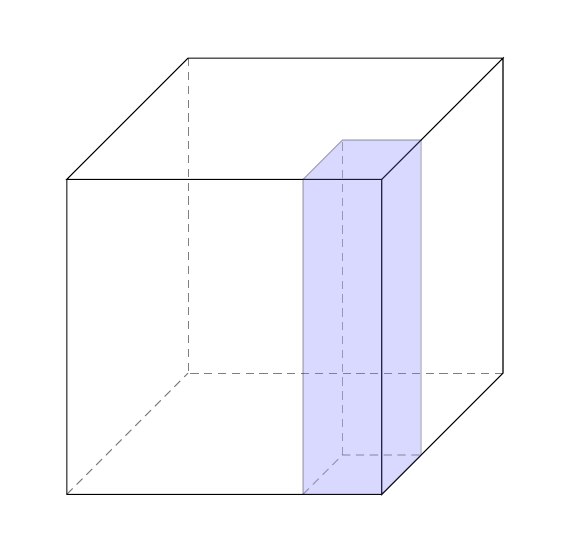
\begin{tikzpicture}
\draw [every edge/.append style={draw=black, densely dashed, opacity=.5}]
(0,0,0) coordinate (o) --
++(-4,0,0) coordinate (a) --
++(0,-4,0) coordinate (b) edge
coordinate [pos=1] (g) ++(0,0,-4) -- ++(4,0,0) coordinate (c) -- cycle
(o) -- ++(0,0,-4) coordinate (d) -- ++(0,-4,0) coordinate (e) edge (g) -- (c) -- cycle
(o) -- (a) -- ++(0,0,-4) coordinate (f) edge (g) -- (d) -- cycle
;
\draw [fill=blue, opacity=.3] (-1,0,0) -- (-.5,.5,0) -- (.5,.5,0) -- (0,0,0);
\draw [fill=blue, opacity=.3]
(.5,.5,0) -- (.5,-3.5,0) -- (0,-4,0) -- (-1,-4,0) -- (-1,0,0) -- (0,0,0);
\draw [opacity=.3, densely dashed] (-1,-4,0) -- (-.5,-3.5,0) -- (.5,-3.5,0);
\draw [opacity=.3, densely dashed] (-.5,-3.5,0) -- (-.5,.5,0);
% just for alignment
\node at (-4.6, -4.5, -.8) {$\phantom{\underline{0}}$};
\node at (2.3, 2.2, 1.4) {$\phantom{\underline{1}}$};
\end{tikzpicture}
\end{document}
















